\documentclass[master=cws,masteroption=gs]{kulemt}

\setup{
  title={Een raamwerk ter ondersteuning van inbraakdetectie in draadloze sensornetwerken},
  author={Christophe Van Ginneken},
  promotor={Prof.\,dr.\,ir.\ Wouter Joosen\and Prof.\,dr.\,ir.\ Christophe Huygens},
  assessor={Ir.\,W. Eetveel\and W. Eetrest},
  assistant={Drs.\,ir.\ Jef Maeri\"en},
  acyear={2013 -- 2014}}

\setup{filingcard,
  translatedtitle={A framework to support intrusion detection in wireless sensor networks},
  udc=621.3,
  shortabstract={Hier komt een heel bondig abstract van hooguit 500
    woorden. \LaTeX\ commando's mogen hier gebruikt worden. Blanco lijnen
    (of het commando \texttt{\string\pa r}) zijn wel niet toegelaten!
    \endgraf}}

%\setup{coverpageonly}

\setup{font=lm}

% Dit mag verwijderd worden voor de af te drukken versie.
\usepackage[pdfusetitle,colorlinks,plainpages=false]{hyperref}

% enkele persoonlijke shortcuts
\newcommand{\TODO}{\textbf{\color{red}TODO}}

\begin{document}

%%!TEX root=masterproef.tex

\begin{preface}

Het is niet iedereen gegeven om op 40-jarige leeftijd een masterproef te mogen
of kunnen maken. De keuze om opnieuw te gaan studeren maak je niet alleen en
vraagt van veel mensen een bijzondere inspanning. Familie en vrienden, maar ook
professoren en assistenten worden geconfronteerd met een ongewone situatie.

Deze masterproef is het resultaat van veel meer dan de afgelopen drie jaren van
hernieuwde studie aan de universiteit van Leuven. Oude en nieuwe ervaringen
gaan hand in hand en hebben geleid tot vragen en antwoorden die groter zijn dan
de som van de afzonderlijke delen.

Dat ik deze masterproef heb kunnen realiseren met de hulp van een fantastisch
team is slechts het topje van de ijsberg. Dat de mensen in dit team ook nog
eens een band hebben met het verleden onderstreept de ondertoon van deze
masterproef.

Professor dr. ir. Wouter Joosen en prof. dr. ir. Christophe Huygens staan
onrechtstreeks weer aan de bakermat van mijn toekomst. Hun passie en
gedrevenheid zijn een bron van inspiratie geweest om dit moeilijke onderwerp
aan te pakken en het tot een goed einde te brengen.

Ofschoon de ongewone situatie soms voor spanningen zorgde, was Jef Maerien de
juiste begeleider, die mijn vlot op deze woelige rivier dikwijls met een klein
manoeuvre op koers wist te houden. Sorry voor mijn soms arrogante attitude en
bedankt voor het behouden vertrouwen. Jouw kritische opmerkingen hebben mij
meer dan eens op de tippen van mijn tenen gehouden en hebben geleid tot betere
resultaten.

Het team bleef niet beperkt tot promotor, co-promotor en begeleider. Tal van
andere professoren en assistenten stonden mij met raad en daad bij wanneer ik
hen benaderde met mijn vragen. Ook buiten de universiteit kon ik steeds rekenen
op mijn vertrouwde klankborden om de juiste weg te vinden. Koen, misschien is
dit slechts het zoveelste fijne project geweest; ik vond het toch extra
speciaal.

Ook al draagt dit werk ogenschijnlijk alleen mijn naam, deze tekst zou nooit
geworden zijn wat hij nu is zonder de talloze uren die mijn team van lezers -
Erik \& Annemie, Bart \& Ans, Pieter \& Else - er hebben in gestoken. Van het
eerste artikel tot de laatste referentie en elke overtollige zinsnede ertussen,
hebben ze gewikt en gewogen en meestal er voor gezorgd dat de tekst er meer dan
vooruit op ging.

Naast mijn persoonlijk gekozen lezers, wil ik ook mijn beide assessoren, \TODO,
bedanken voor de tijd die ze namen om dit werk te evalueren. Ik hoop werkelijk
dat wij later de gelegenheid zullen vinden om alsnog van gedachten te wisselen.
Uw bemerkingen kunnen mij immers helpen om bepaalde aspecten nog beter uit te
werken, want voor mij is deze masterproef geen eindbestemming.

Maar ondanks de steun van heel dit team, was deze masterproef nooit gelukt
zonder een team op het thuisfront. Opnieuw drie jaar gaan studeren overstijgt
een klassieke dagtaak en legt een veel grotere druk op een gezin dan we voor
aanvang hadden kunnen inschatten. Zo heeft mijn \emph{soulmate} Kristien elke
seconde van de afgelopen drie jaar, elke druppel zweet en tranen mee
doorgemaakt, hebben ouders en schoonouders op de meest onmogelijke momenten
ingesprongen om mij tijd en ruimte te geven om dit te realiseren en moesten we
meer dan eens beroep doen op vrienden en buren om allerhande elementaire
karweien voor ons te doen. Het is hartverwarmend om te ervaren hoeveel mensen
de afgelopen drie jaar meegeleefd hebben.

Tot slot zijn er nog twee mensen die echt een hele dikke knuffel verdienen. Van
iedereen begrijpen zij misschien het minst wat papa gedaan heeft de afgelopen
jaren en waarom er zo weinig tijd voor hen overbleef. Eline en Arjen, mijn
lieve schatten, bedankt dat jullie soms zo begripvol waren en me dikwijls
opnieuw moed hebben gegeven om toch door te gaan.

\bigskip

Bedankt!

\end{preface}


%\tableofcontents*

%%!TEX root=masterproef.tex

\begin{abstract}

Draadloze sensornetwerken treden met rasse schreden onze persoonlijke
levenssfeer binnen. Een afdoende beveiliging tegen inbraken, moet garanties
kunnen bieden dat deze vooruitgang zelf geen bedreiging wordt. Preventie is een
eerste stap, maar niet alle inbraken kunnen verijdeld worden. Soms moeten we
genoegen nemen met het kunnen detecteren van inbraken om ons er in toekomstige
situaties beter tegen te wapenen.

Het introduceren van inbraakdetectie in draadloze sensornetwerken resulteert al
snel in een gevecht om middelen: een draadloze sensorknoop beschikt over een
beperkte autonomie en moet zijn energie optimaal benutten. Hieraan
inbraakbeveiliging toevoegen, vraagt veel van de beschikbare middelen en
bedreigt daarmee de kans om opgenomen te worden in het uiteindelijke ontwerp
van elk nieuwe draadloze sensorknoop.

Indien het probleem niet kan vermeden worden, moeten we trachten het
draaglijker te maken. Deze masterproef wil zowel de druk op de middelen van de
sensorknopen verlichten als de bijkomende economische druk op de ontwikkeling,
die de introductie van inbraakdetectie met zich meebrengt, reduceren.

Om dit te realiseren wordt een domeinspecifieke taal voorgesteld die
onderzoekers in staat stelt om algoritmen voor inbraakdetectie op een formele
en platformonafhankelijke manier te defini\"eren. Deze eerste stap ontslaat
ontwikkelaars van nieuwe sensornetwerken van de taak om onderzoeksliteratuur te
doorworstelen en algoritmen uit deze teksten te puren.

Een formele beschrijving laat verder toe om deze op geautomatiseerde wijze te
benaderen. Zo wordt het mogelijk om door middel van codegeneratie de algoritmen
automatisch om te zetten in platformspecifieke programmacode, zo georganiseerd
dat de middelen van de sensorknoop zo optimaal mogelijk benut worden.

Dankzij het vrijwaren van de middelen van de sensorknoop en het reduceren van
de economische kost, wordt het mogelijk om meer inbraakpogingen te detecteren.

De initi\"ele testen met een prototype code generator zijn veel belovend en
bevestigen de intu\"itie dat een goede organisatie van verschillende
detectiealgoritmen kan leiden tot een beter gebruik van de middelen van een
sensorknoop.

Zowel de domeinspecifieke taal als van de code generator dienen verder
onderzocht te worden en de testen moeten op grotere schaal uitgewerkt worden.
De realisatie van een ecosysteem rond de geformaliseerde detectiealgoritmen is
een andere belangrijke richting die nagestreefd kan en moet worden, waar vooral
het onderzoeksdomein bij zou baten.

\end{abstract}


%\listoffigures
%\listoftables
%\listoffiguresandtables

%%!TEX root=masterproef.tex

\chapter{Lijst van afkortingen en symbolen}
\section*{Afkortingen}

\TODO

\begin{flushleft}
  \renewcommand{\arraystretch}{1.1}
  \begin{tabularx}{\textwidth}{@{}p{12mm}X@{}}
    LoG   & Laplacian-of-Gaussian \\
    MSE   & Mean Square error \\
    PSNR  & Peak Signal-to-Noise ratio \\
  \end{tabularx}
\end{flushleft}
\section*{Symbolen}

\begin{flushleft}
  \renewcommand{\arraystretch}{1.1}
  \begin{tabularx}{\textwidth}{@{}p{12mm}X@{}}
    42    & ``The Answer to the Ultimate Question of Life, the Universe, and Everything'' \\
    $c$   & Lichtsnelheid \\
    $E$   & Energie \\
    $m$   & Massa \\
    $\pi$ & Het getal pi \\
  \end{tabularx}
\end{flushleft}


\mainmatter

%!TEX root=masterproef.tex

\chapter{Inleiding}
\label{inleiding}

Ze hebben de voorpagina van de krant dan misschien nog niet gehaald, de opmars
van draadloze sensornetwerken (\emph{Wireless Sensor Networks}) (WSN) in ons
dagelijks leven is niet meer te stoppen. Na de revolutie van de persoonlijke
computer, de smartphone en het tablet vinden nu onafhankelijke, minuscule
computers hun weg naar allerlei alledaagse dingen en plaatsen in ons leven.
Deze netwerken kunnen met hun sensoren de kleinste wijzigingen in hun omgeving
optekenen. Via een draadloos netwerk staan de sensoren in verbinding met elkaar
en de buitenwereld. Zo leveren ze hun informatie af, waardoor wij op elk moment
precies weten hoe warm het in elke kamer van ons huis is of welke groenten nog
in de koelkast liggen. Het lijkt nog science fictie, maar deze toekomst is heel
wat dichterbij dan we vermoeden.

Om deze technologie te omarmen en ons leven verder in te richten met deze
ondersteunende hulp, moeten we ons er van vergewissen dat deze technologie
betrouwbaar en veilig is. Als enkele sensoren in ons huis slechts een kleine
stap met weinig potenti\"ele, problematische gevolgen lijkt, moeten we ons toch
bezinnen en beseffen dat al deze kleine computers zeer interessante
inbraakmogelijkheden bieden aan anderen met minder positieve bedoelingen.

Misschien wil de concurrent van de producent van onze yoghurt zijn collega wel
in diskrediet brengen door er voor te zorgen dat onze slimme koelkast het
nalaat ons te verwittigen dat de yoghurt vervallen is. Misschien vindt de
gasleverancier het wel leuk om, wanneer we niet thuis zijn, de thermostaat een
graadje hoger te zetten.

De mogelijkheden van draadloze sensornetwerken lijken eindeloos en ze kunnen de
kwaliteit van ons leven ingrijpend veranderen. Ze mogen echter geen bijkomende
bedreiging introduceren. In deze masterproef duiken we in de wereld van
draadloze sensornetwerken en willen we nagaan of en hoe we deze kunnen voorzien
van bescherming tegen minder goede bedoelingen.

Sectie \ref{section:wsn} introduceert draadloze sensornetwerken. Hoe zijn ze
opgebouwd? Wat zijn de mogelijkheden en beperkingen? 

Sectie \ref{section:beveiligen} legt de nadruk op beveiliging: Wat zijn de
gevaren? Hoe kunnen deze vastgesteld worden? Hoe kunnen sensorknopen beschermd
worden?

Sectie \ref{section:probleem} brengt beide aspecten samen en vat de
probleemstelling samen.

Sectie \ref{section:doelstelling} legt tot slot kort de doelstelling van deze
masterproef uit.

\section{Draadloze sensornetwerken}
\label{section:wsn}

Sinds de late jaren '90 zijn draadloze sensornetwerken een bron geweest voor
een overvloed aan onderzoek. Binnen en buiten universiteiten werden deze
netwerken ingezet voor allerhande toepassingen: van het opvolgen van
microklimaten bij het telen van gewassen \citep{baggio2005wireless} tot het
vastleggen van vulkanische activiteit \citep{werner2005monitoring} en het
opvolgen van overstromingsgebieden \citep{hughes2006gridstix}.

Wat moeten we ons eigenlijk voorstellen bij een draadloos sensornetwerk? We
bekijken kort de sensorknopen, waarmee het netwerk wordt opgebouwd. Vervolgens
belichten we het draadloze netwerk dat de knopen in staat stelt om met elkaar
en met de buitenwereld te communiceren.

\subsection{Sensorknopen}

Sensorknopen zijn in essentie zeer eenvoudige computers. Ze worden typisch
opgebouwd rond een microcontroller (\mcu). Dit is een digitaal ontwerp dat
zowel een processor als geheugen en invoer- en uitvoerkanalen bevat op \'e\'en
ge\"integreerde schakeling. Ze worden daarom ook wel \emph{systeem-op-een-chip}
(\emph{System-on-Chip}) (SoC) genoemd. Figuur \ref{fig:motes} toont enkele
typische sensorknopen.

\begin{figure}[ht]
\centering
\begin{subfigure}{.24\textwidth}
  \centering
  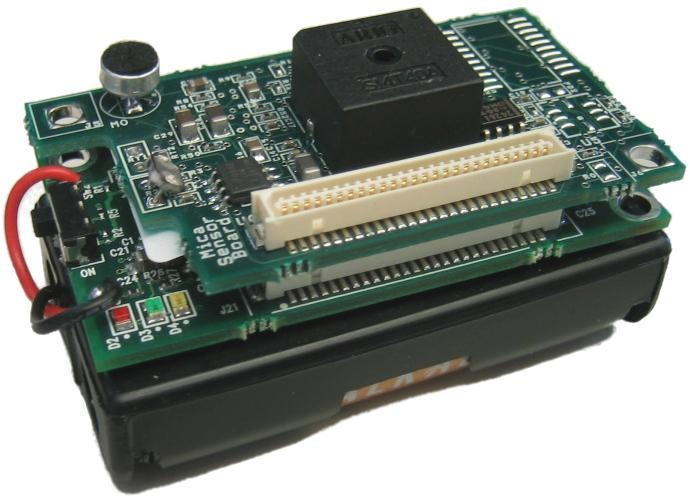
\includegraphics[width=.9\linewidth]{./resources/mica2.jpg}
  \caption{Mica2}
  \label{fig:mica2}
\end{subfigure}
\begin{subfigure}{.24\textwidth}
  \centering
  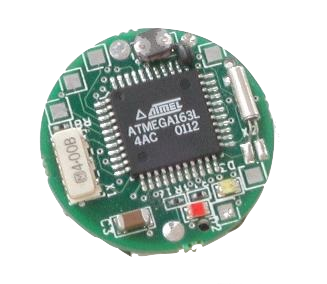
\includegraphics[width=.9\linewidth]{./resources/dot.png}
  \caption{Dot}
  \label{fig:dot}
\end{subfigure}
\begin{subfigure}{.24\textwidth}
  \centering
  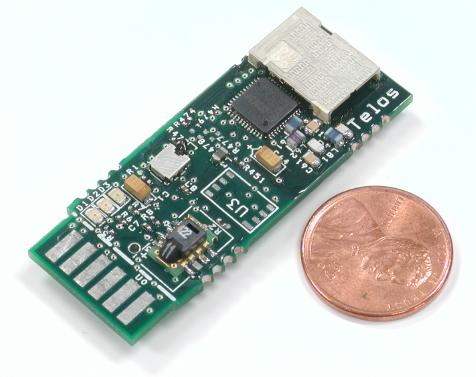
\includegraphics[width=.9\linewidth]{./resources/telos.jpg}
  \caption{Telos}
  \label{fig:telos}
\end{subfigure}
\begin{subfigure}{.24\textwidth}
  \centering
  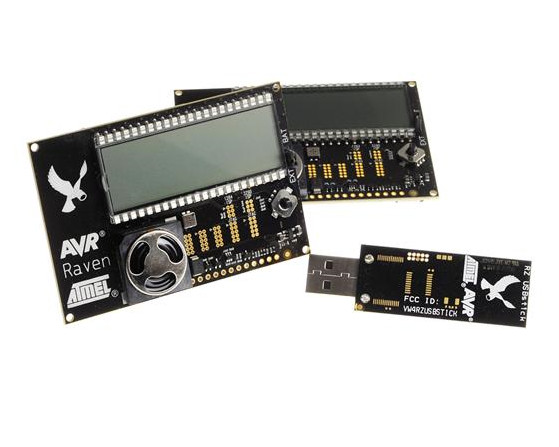
\includegraphics[width=.9\linewidth]{./resources/raven.jpg}
  \caption{AVRraven}
  \label{fig:raven}
\end{subfigure}
\caption{Voorbeelden van sensorknopen}
\label{fig:motes}
\end{figure}

Naast de \mcu heeft een typische sensorknoop tevens een draadloze radio. Je kan
dit vergelijken met de Wi-Fi verbinding die je tegenwoordig in de meeste
computers of smartphones vindt. Voor sensorknopen wordt echter meestal
geopteerd voor een draadloze radio die een minimum aan energie probeert te
verbruiken. Verschillende nieuwe draadloze netwerkstandaarden zijn de laatste
jaren op de voorgrond getreden. De bekendste zijn 6LoWPAN \citep{rfc:6282} en
ZigBee \citep{alliance2012zigbee}. In de volgende paragrafen bekijken we ZigBee
van naderbij; enerzijds omwille van de toepassing in deze masterproef, maar ook
omwille van de voorbeeldfunctie die het kan aannemen voor deze groep van
draadloze standaarden.

\subsection{ZigBee}
\label{subsection:zigbee}

ZigBee zelf is een laag bovenop de netwerklaag gekend als IEEE 802.15.4
\citep{ieee2009802.15.4}. Deze voorziet standaarden op vlak van energiegebruik,
adressering, foutcorrectie, vormgeving van berichten\dots en vormt zo de
fundamenten voor zgn. \emph{low-rate wireless personal area networks}
(LR-WPAN). ZigBee voegt hieraan nog drie belangrijke eigenschappen toe:
routering, ad-hoc netwerkcreatie en zelfherstellende maasnetwerken (\emph{mesh
networks}) \citep{oreilly2010buildingwsn}.

Een ZigBee-netwerk wordt opgebouwd door knopen die elk \'e\'en van drie
verschillende functies kunnen innemen: co\"ordinator, router of eindknoop.

\begin{description}

  \item[Co\"ordinator] Elk netwerk heeft \'e\'en \emph{co\"ordinator}. Deze
  knoop is verantwoordelijk voor het samenbrengen van het netwerk en definieert
  de eigenschappen, bv. met betrekking tot de beveiliging.

  \item[Router] Een \emph{router} stelt andere knopen in staat om met elkaar te
  communiceren. Deze knopen zijn daarom meestal voorzien van een permanente
  stroomvoorziening, omdat ze zich in tegenstelling tot \emph{eindknopen},
  wegens hun communicatieondersteunende rol, niet in een slaapstand kunnen
  zetten.

  \item[Eindkknoop] \emph{Eindknopen}, tot slot, kunnen zich louter verbinden
  met een netwerk, er berichten via versturen en berichten voor zichzelf
  ontvangen. Het is niet de bedoeling om berichten van andere knopen voor
  andere knopen door te sturen. Typisch trachten ze ook hun energieverbruik te
  minimaliseren door hun draadloze radio zoveel mogelijk uit te schakelen.
  Hierdoor worden ze op dat moment onbereikbaar. Het is dankzij \emph{routers},
  die berichten voor de \emph{eindknopen} tijdelijk opslaan, dat ze toch
  berichten kunnen ontvangen.

\end{description}

\subsection{Netwerktopologie en -adressen}
\label{subsection:topologie}

Met knopen kunnen verschillende netwerktopologie\"en gebouwd worden. Figuur
\ref{fig:topologie} geeft een overzicht van de mogelijkheden.

\begin{description}

  \item[Paar] In zijn eenvoudigste vorm bestaat een netwerk uit een
  co\"ordinator en een eindknoop. Deze minimalistische vorm is slechts een
  theoretische mogelijkheid ter volledigheid van de mogelijkheden.
  
  \item[Ster] Wanneer meerdere eindknopen verbonden zijn met dezelfde
  co\"ordinator, vormen zij een stertopologie. Alle communicatie verloopt via
  de centrale co\"ordinator.
  
  \item[Maasnetwerk] In een maasnetwerk worden routers ingeschakeld om
  communicatie via verschillende wegen mogelijk te maken. Eindknopen zijn
  verbonden met deze routers of met de co\"ordinator. Routers en co\"ordinator
  kunnen berichten ontvangen van eindknopen en deze versturen naar andere
  eindknopen, al dan niet via andere routers.
  
  \item[Clusterboom] Een speciale vorm van een maasnetwerk is een clusterboom.
  Hierbij vormen groepen van eindknopen en een router een cluster. De router is
  verbonden met de co\"ordinator, eventueel opnieuw via andere routers, en zo
  wordt een boomstructuur gevormd. De routers die de clusters van eindknopen
  realiseren worden ook clusterhoofden genoemd.
  
\end{description}

\begin{figure}[ht]
  \centering
  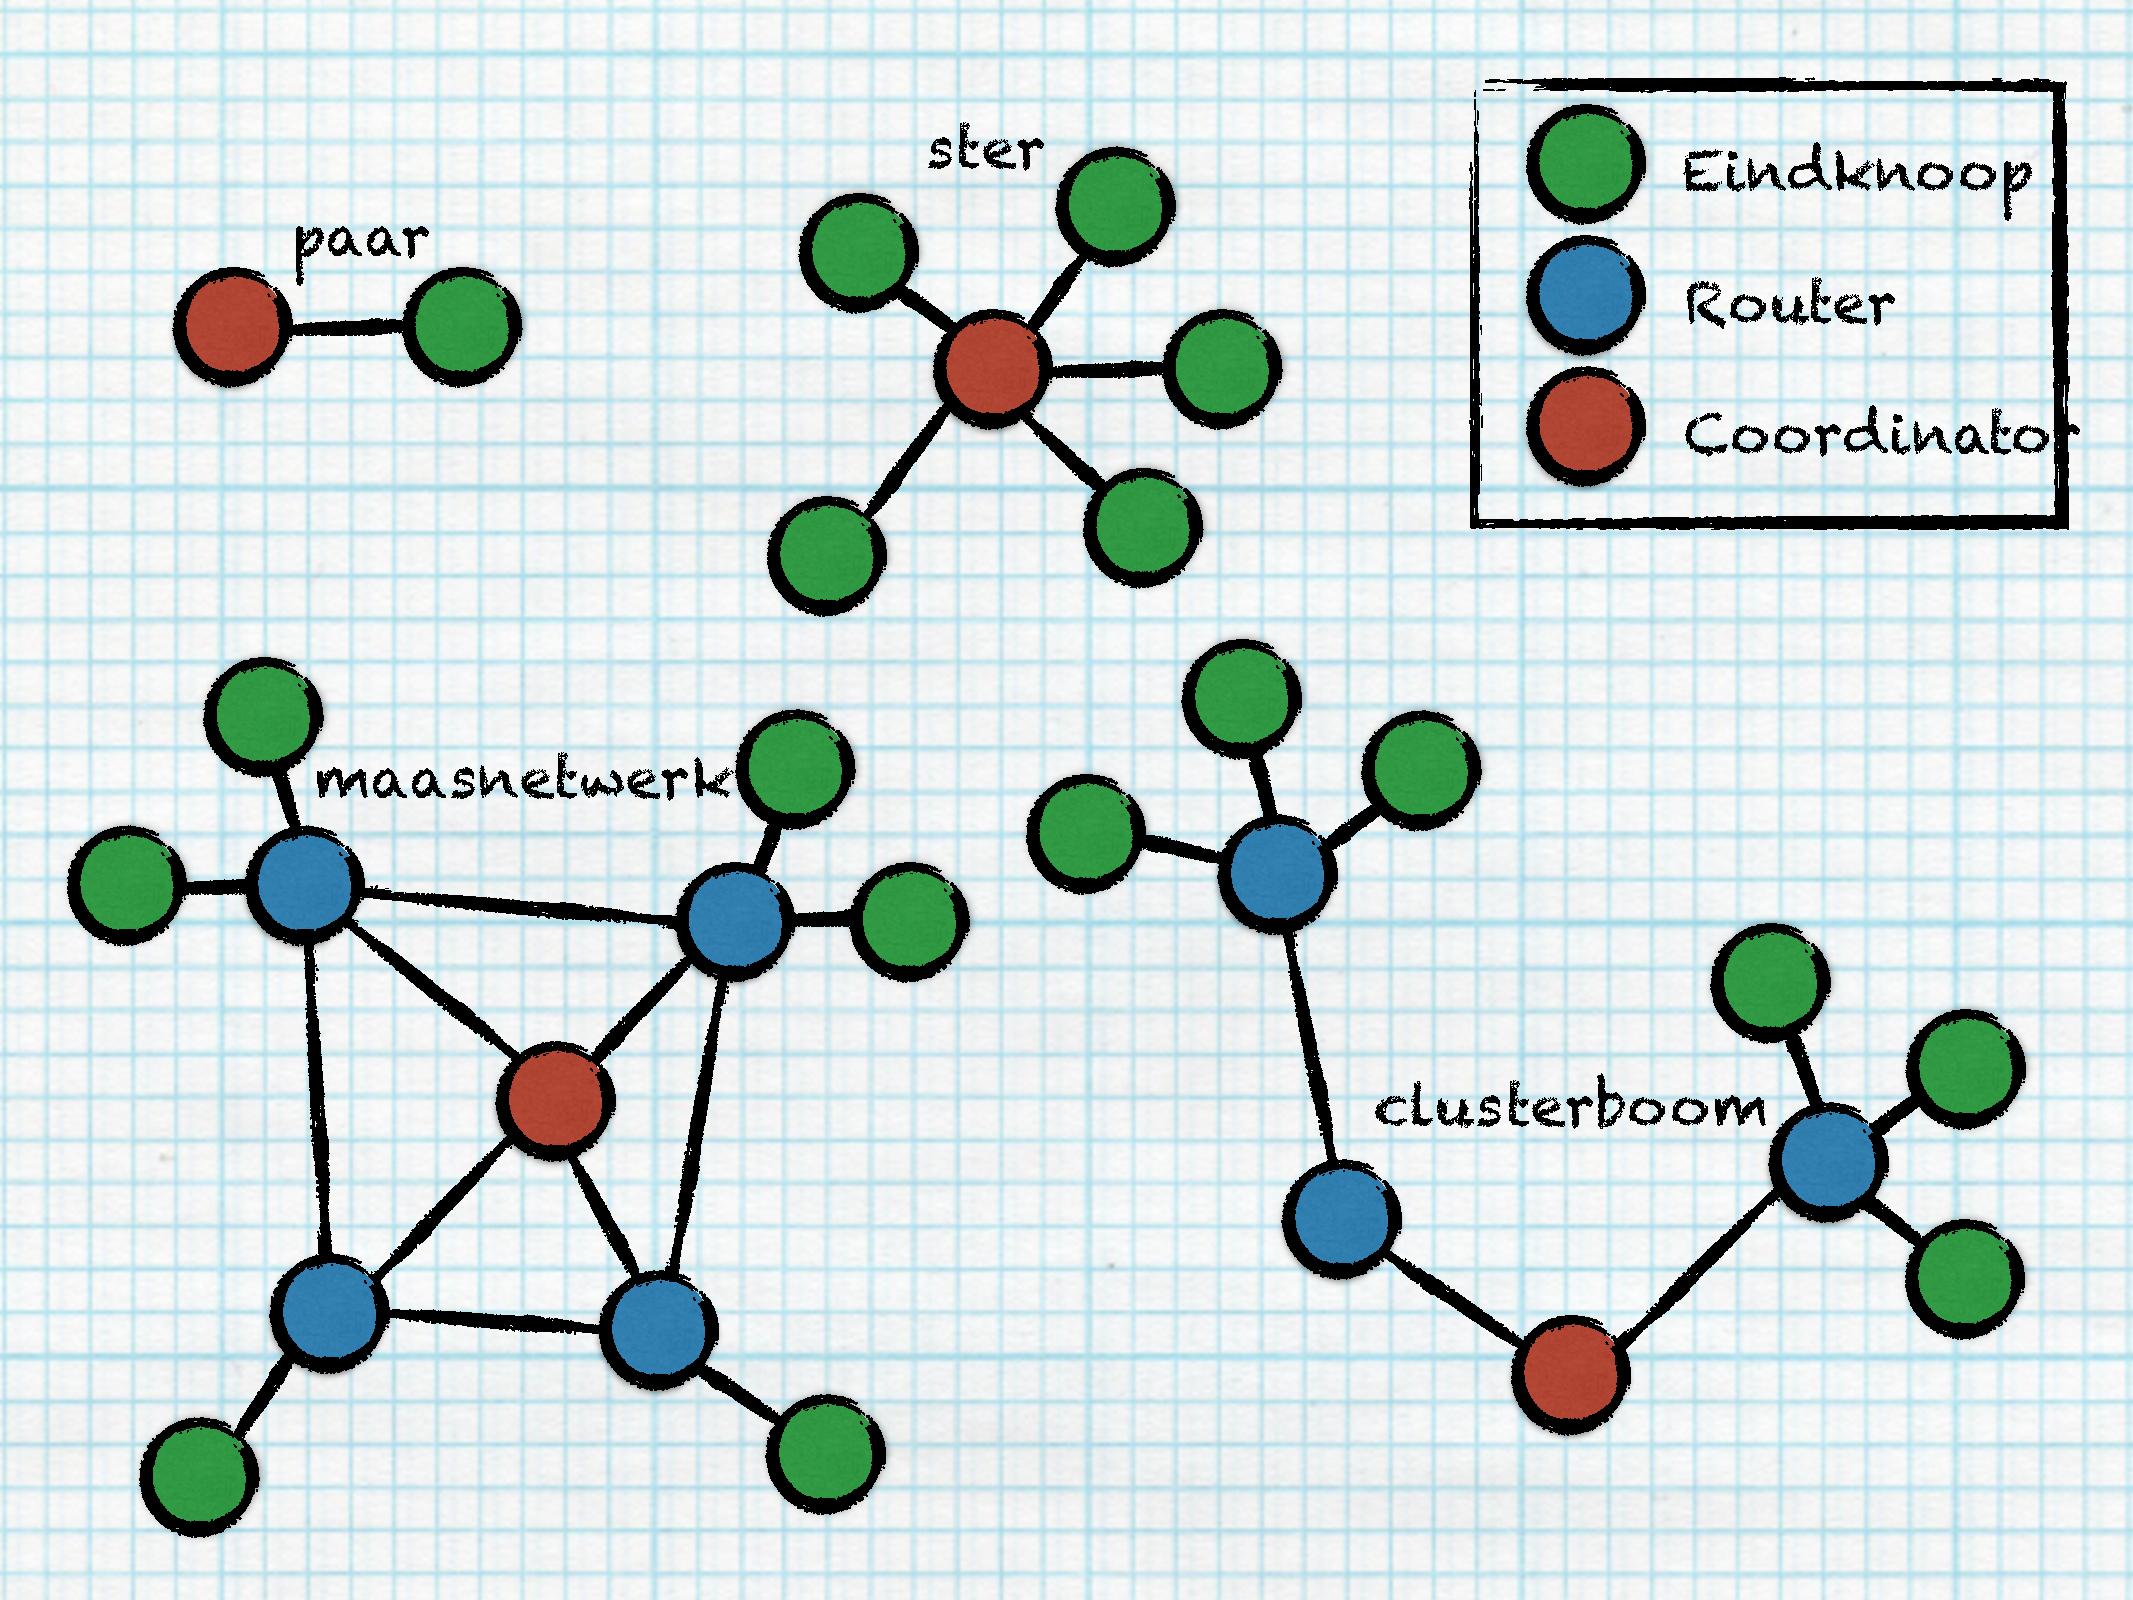
\includegraphics[width=0.7\linewidth]{resources/topology.pdf}
  \caption[Verschillende mogelijke netwerktoplogie\"en]{Verschillende mogelijke
  netwerktoplogie\"en (Bron:\citep{oreilly2010buildingwsn})}
  \label{fig:topologie}
\end{figure}

Het lijkt evident, maar elke knoop, in eender welke topologie, heeft een eigen,
uniek adres, eigenlijk meerdere. Zo heeft een ZigBee-knoop een uniek adres
binnen het netwerk waaraan het deelneemt. Dit adres wordt door de co\"ordinator
van het netwerk toegekend aan een knoop wanneer deze toetreedt tot het netwerk.
Dit \emph{netwerkadres} bestaat uit 16 bits en laat dus toe om 65534 (uit
$2^{16} = 65536$) verschillende adressen toe te kennen. Het adres
\ttt{0x0000}\footnote{We hanteren voor de notatie van adressen de hexadecimale
voorstelling. Elk cijfer stelt een groep van 4 bits voor. 4 groepen stellen zo
een 16 bit adres voor.} reserveert de co\"ordinator voor zichzelf en het adres
\ttt{0xFFFE} wordt typisch gebruikt als het zgn. \emph{broadcast adres}, het
adres waarnaar een bericht gestuurd wordt dat bij alle andere knopen dient
afgeleverd te worden.

Daarnaast heeft elke ZigBee-radio ook een adres dat gegarandeerd overal uniek
is. Dit bestaat uit 64 bits en wordt samengesteld uit twee delen: een eerste
deel beslaat de eerste 32 bits en is voorbehouden voor een unieke identificatie
van de producent. De volgende 32 bits is een uniek nummer binnen de productie
van de producent. Een netwerk zal veelal uit sensoren met dezelfde draadloze
radio's bestaan. Het is daarom logisch dat er gebruik gemaakt wordt van een
\emph{netwerkadres}, dat slechts 16 bits groot is en dus een aanzienlijke
besparing aan geheugen kan opleveren.

Naast de adressen van de knopen is er ook nog het zogenaamde \emph{personal
area network (PAN)} adres. Dit is een unieke identificatie van het netwerk dat
door de co\"ordinator georganiseerd wordt. Ook dit is een 16 bit adres en laat
dus toe om 65536 netwerken op te bouwen.

Tot slot kunnen ZigBee-radio's ook gebruik maken van 12 verschillende
\emph{kanalen}, zodat de volledige adresstructuur bestaat uit een kanaal, een
PAN adres en een netwerkadres.

\section{Beveiligen van sensorknopen}
\label{section:beveiligen}

Het beveiligen van sensorknopen is, in tegenstelling tot de beveiliging van
klassieke computers, bijzonder moeilijk. De computers waar onze emails, foto's
en andere kostbare documenten opgeslagen zijn, zijn uitgerust met een
virusscanner, firewall\dots Dit is mogelijk omdat ze voorzien zijn van een
constante stroomvoorziening, krachtige processor en veel geheugen. Ze worden
tevens fysiek beschermd door ons huis of het datacenter van onze leverancier
van internetdiensten.

In \citep{dargie2010fundamentals} wordt een goed overzicht gegeven van de
uitdagingen die het beveiligen van WSN met zich meebrengen, in vergelijking met
klassieke netwerken. Een sensorknoop heeft geen constante stroomvoorziening en
moet het veelal stellen met een zeer beperkte batterij. Verder ligt de
sensorknoop meestal letterlijk \emph{ten velde} en is hij voor nagenoeg
iedereen fysiek toegankelijk.

Er is ook geen centraal punt waar alle communicatie gegarandeerd passeert. Het
enige communicatiemedium is het draadloze netwerk en via die weg kan men steeds
rechtstreeks contact leggen met elke afzonderlijke knoop, zonder dat de
meerderheid van andere knopen dit ooit merkt. Tot slot is mogen we niet
vergeten dat een draadloos communicatiemedium inherent fouten introduceert, en
dat berichten verloren kunnen gaan.

\subsection{CIA, AAA en andere beveiligingsprincipes}
\label{subsection:cia}

Beveiliging is een zeer ruim begrip dat veel aspecten overspant. Het is
belangrijk dit voor ogen te houden wanneer we over beveiliging spreken.
Theoretische modellen kunnen hierbij helpen. In deze sectie introduceren we
enkele van deze modellen die kunnen helpen om over beveiliging te praten.

Wanneer men spreekt over het beveiligen van computers en netwerken, wordt
dikwijls gerefereerd naar het CIA-beveiligingsmodel. Dit letterwoord staat
voor: vertrouwelijkheid (\emph{confidentiality}), integriteit en
beschikbaarheid (\emph{availability}).

\begin{description}

  \item[Vertrouwelijkheid] Om \emph{vertrouwelijkheid} te garanderen moet
  beveiliging de nodige voorzieningen treffen om er voor te zorgen dat bv. een
  bericht enkel door de bedoelde bestemmeling kan begrepen worden.
  
  \item[Integriteit] Onder \emph{integriteit} verstaat men het principe dat dat
  bericht dan weer niet mag gewijzigd kunnen worden, of dat de bedoelde
  bestemmeling van het bericht ten minste kan valideren dat er aan het bericht
  niets gewijzigd is. 
  
  \item[Beschikbaarheid] Maar beveiliging moet ook de \emph{beschikbaarheid}
  van onderdelen van het netwerk garanderen, om er zeker van te zijn dat dit
  laatste zijn diensten kan blijven aanbieden.

\end{description}

Het CIA-model is zonder meer een belangrijke basis, maar er ontbreken nog veel
belangrijke aspecten. In \citep{rfc:3198} wordt een gestandaardiseerde
terminologie voorgesteld voor het defini\"eren van een beveiligingsbeleid.
Naast de drie hoofdpijlers van het CIA-model vinden we zo ook nog een ander
belangrijk model, namelijk het AAA model voor autorisatie bij
internet-gerelateerde diensten (\emph{triple A}) \citep{rfc:2904}. De afkorting
staat voor authenticatie, autorisatie en vaststellen (\emph{accounting})

\begin{description}

  \item[Authenticatie] Via \emph{authenticatie} kan de identiteit van een
  gebruiker of apparaat vastgesteld worden, zodat eenduidig kan bepaald worden
  van wie bv. een bericht in het netwerk komt.
  
  \item[Autorisatie] \emph{Autorisatie} is daarentegen het proces waarbij
  nagegaan wordt of een gebruiker waarvan de authenticiteit is vastgesteld, een
  bepaalde handeling \emph{mag} uitvoeren.
  
  \item[Vaststellen] Ten slotte biedt het \emph{vaststellen} van alle
  gebeurtenissen en beslissingen binnen het beveiligde domein, een belangrijke
  bron van informatie om een beleid verder te verfijnen en eventueel bij te
  sturen.

\end{description}

In het kader van beveiliging wordt gesproken over een \emph{beleid}
(\emph{policy}), waarin de regels zijn opgenomen waaraan alle spelers binnen
het te beveiligen domein zich dienen te houden. Het AAA-model hanteert een
beleid als zijn centrale gegeven en definieert componenten zoals een
\emph{policy information point} (PIP), \emph{policy decision point} (PDP) en
een \emph{policy enforcement point} (PEP). Deze componenten kunnen aanduiden
waar de verantwoordelijkheid ligt om respectievelijk de juiste informatie aan
te leveren omtrent het beleid, beslissingen te treffen volgens het beleid en
deze beslissingen effectief uit te voeren.

\begin{description}

  \item[Onweerlegbaarheid] Naast deze aspecten, is er ook nog het principe van
  onweerlegbaarheid (\emph{non-repudiation}). Door garanties omtrent
  \emph{onweerlegbaarheid} in te bouwen, kan een ontvanger er zeker van zijn
  dat een zender van een bericht dit bericht effectief verstuurd heeft.

\end{description}

Een aantal gekende technieken bieden klassiek oplossingen voor verschillende
van de hoger vermelde principes: digitale handtekeningen kunnen helpen bij het
garanderen van de \emph{authenticiteit}, \emph{onweerlegbaarheid} en
\emph{integriteit} van een boodschap. Cryptografie kan logischerwijs de
\emph{vertrouwelijkheid} van berichten garanderen, maar kan ook, aan de hand
van publieke en private sleutels, de \emph{authenticiteit} vaststellen.
Berichten kunnen alleen met de andere sleutel van het paar versleuteld worden.

In hoofdstukken \ref{chapter:achtergrond} en \ref{chapter:probleemstelling}
gaan we dieper in op de typische eigenschappen van sensorknopen en belichten we
tal van beveiligingsrisico's waaraan een WSN blootgesteld zijn. Aan de hand van
de zonet beschreven principes zullen we zien dat een WSN inherent moeilijk te
beveiligen is en dat het nagenoeg onmogelijk is om inbraken te vermijden.

\subsection{Inbraakdetectie}
\label{subsection:detection}

Indien het vermijden van inbraken nagenoeg onmogelijk is, moet een belangrijke
tweede beveiligingslinie opgetrokken worden: inbraakdetectie.

Indien we niet weten dat een inbraak heeft plaatsgevonden, zullen we enkel een
vals gevoel van veiligheid hebben. Het is niet omdat we het niet weten, dat ze
er niet zijn. Misschien moeten we zelfs durven stellen dat het belangrijker is
om meer te weten dan te vermijden.

Inbraakdetectie is typisch de stille vennoot in een beveiligingsverhaal. Daar
waar bv. een firewall of authenticatieserver actief toegang ontzegt, zal een
inbraakdetectiesysteem (IDS) typisch geen actieve rol spelen. Het IDS zal
eerder bewijsmateriaal verzamelen om een inbraakpoging te documenteren. Uit
deze informatie kunnen dan bijsturingen aan het beleid aangebracht worden,
waardoor actieve componenten in de toekomst wel in staat zijn om gelijkaardige
inbraakpogingen te verijdelen.

Deze architectuur legt al snel een belangrijk pijnpunt bloot: in een klassiek
netwerk wordt het netwerk beschermd aan de rand. De firewall schermt het
interne netwerk af van aanvallen van buiten. Als een spreekwoordelijke muur van
vuur wordt elke toegang tot het netwerk gelouterd en ongewenste berichten
worden onherroepelijk \emph{verbrand} v\'o\'or ze het netwerk kunnen betreden.

Het IDS wordt daarom typisch ook op het interne netwerk aangesloten daar waar
alle netwerkverkeer dat door de firewall wordt doorgelaten, passeert. Aanvallen
die toch nog door de firewall geraken, kunnen nog door het IDS gedetecteerd
worden.

Dit lijkt op het eerste zicht een tegenspraak. Indien het IDS deze aanvallen
kan detecteren, waarom wordt deze kennis dan niet gebruikt op het niveau van de
firewall? De reden ligt in de natuur van de firewall. Deze werkt immers
hoofdzakelijk op netwerkniveau en bekijkt elk netwerkpakket op zich. Aanvallen
zijn soms een samengang van verschillende pakketten, die typisch op zich zelfs
perfect legaal zijn. Het draait hier hoofdzakelijk om de inhoud van de
pakketten en de analyse vraagt dikwijls een kennis van de toepassingen waarmee
gecommuniceerd wordt. Soms kan slechts aan de inhoud van antwoorden uit het
interne netwerk opgemaakt worden dat er een inbraak plaatsgevonden heeft. Deze
complexiteit is te groot om op het niveau van een firewall te realiseren.

De resultaten van een IDS zullen dikwijls eerder leiden tot verbeteringen aan
de toepassingen binnen het interne netwerk, zodat deze niet meer vatbaar zijn
voor het soort inbraken dat gedetecteerd werd.

Wanneer we dit nu afspiegelen op een WSN, merken we dat enkele fundamentele
principes zo'n architectuur onmogelijk maken: een WSN heeft geen afgebakende
netwerkrand, er is geen uniek punt waar alle netwerkverkeer passeert en waar
een firewall zou kunnen ge\"introduceerd worden, laat staan dat er een manier
zou zijn om al het interne verkeer op \'e\'en enkele plaats te analyseren.

Binnen een WSN is het letterlijk elke knoop voor zichzelf: elke knoop kan
immers van buitenaf benaderd worden zonder dat een aanvaller moet passeren
langs een centraal controlepunt.

\section{Probleemstelling}
\label{section:probleem}

WSN en sensorknopen op zich zijn geen makkelijke klanten wat beveiliging
betreft. Enerzijds hebben ze onvoldoende middellen om zich te beschermen en
anderzijds is hun situatie zo dat het letterlijk elke knoop voor zichzelf is en
dat ze nauwelijks kunnen vertrouwen op hun collega's.

In dit kader moeten gebruikers van een WSN eisen dat er voldoende garanties
worden gegeven zodat ze zich voldoende verzekerd voelen om intieme informatie
toe te vertrouwen aan deze netwerken.

Aangezien het haast onmogelijk is om inbraakpogingen te verijdelen is het van
groot belang dat men in staat is om ze ten minste vast te stellen. Het
introduceren van een IDS in het WSN is echter een directe aanval op de
essenti\"ele functionaliteit van een sensorknoop, waardoor de mogelijkheden
sterk beperkt worden.

\section{Doelstelling}
\label{section:doelstelling}

Zoals we zullen zien in sectie \ref{section:related}, ligt in de literatuur
betreffende ``inbraakdetectie in draadloze sensornetwerken'' de nadruk in
hoofdzaak op het detecteren van specifieke aanvallen of het vaststellen van
anomalie\"en in het verwachte gedrag van sensorknopen en/of het netwerk dat hen
verbindt.

Deze werken stellen tevens dat het een nagenoeg onmogelijke taak is om alle
benodigde detectiemechanismen effectief te implementeren. Dit is logisch,
gegeven de beperkte middelen die sensorknopen ter beschikking hebben. Zo zou
bv. een exhaustieve lijst van aanvalspatronen slechts in sensorknopen met een
groot geheugen opgeslagen kunnen worden en zouden de berekeningen die nodig
zijn om bepaalde anomalie\"en te detecteren gewoonweg te veel energie
verbruiken.

Als in dit stadium van onderzoek naar systemen om inbraken te detecteren het
niet mogelijk is om een sluitend IDS voor een WSN te ambi\"eren, lijkt het
opportuun om een stap terug te zetten en de focus te leggen op de middelen die
nodig zijn om de reeds beschreven, en mogelijk ook toekomstige algoritmen, te
realiseren. Is het mogelijk om een kader te cre\"eren dat een ontwikkelaar van
een sensorknoop in staat stelt om een selectie van de in de literatuur
beschreven oplossingen te implementeren? Kan hij een IDS toevoegen aan zijn WSN
zonder een diepgaande analyse van de onderzoeksliteratuur en zonder zich zorgen
te moeten maken over de onderliggende interactie met andere knopen, het
vergaren en opvragen van informatie op systeem-niveau\dots?

Deze masterproef wil zo'n kader ontwerpen, een prototype implementeren en de
impact bepalen. Daartoe bekijken we eerst enkele typische voorbeelden van
inbraakdetectiealgoritmen, waaruit de functionele en technische vereisten
gedistilleerd worden. Vervolgens stellen we een architectuur voor die aan deze
vereisten kan voldoen. Aan de hand van een prototype gaan we tot slot na wat de
impact is met betrekking tot geheugen, rekenkracht en het gebruik van de
draadloze radio.

De voordelen van een raamwerk zijn legio: een herbruikbaar raamwerk neemt
zorgen, gemeenschappelijk aan de verschillende oplossingen, weg en kan zorgen
voor een betere implementatie. Door middel van een goedgekozen technische
architectuur kan tevens platformonafhankelijheid nagestreefd worden.

%!TEX root=masterproef.tex
\chapter{Achtergrond}
\label{chapter:achtergrond}

In dit hoofdstuk wordt het kader geschetst waarbinnen deze thesis op zoek gaat
naar antwoorden. Enerzijds wordt in sectie \ref{section:landscape} het
landschap van draadloze sensornetwerken in kaart gebracht: wat typeert en
onderscheid hen van andere netwerken? Waarom is het vaststellen van inbreuken
een belangrijk onderzoeksdomein?

Anderzijds wordt in sectie \ref{section:related} ingegaan op een groot aanbod
aan gerelateerd onderzoek. Een belangrijke doelstelling van deze thesis is het
in kaart brengen van de mogelijkheden en beperkingen betreffende reeds
beschreven methodes om inbreuken vast te stellen.

De verschillende beschreven methodes worden gecatalogeerd en gegroepeerd op
basis van verschillende eigenschappen. Op basis van dit overzicht wordt
vervolgens een inschatting gemaakt van de mogelijke dekking die kan bereikt
worden met de bestaande oplossingen.

Bij de beschrijving van de verschillende oplossingen zal tevens kritisch
nagegaan worden in hoeverre de oplossingen in een realistische situatie
effectief bijdragen tot het detecteren van inbreuken in het netwerk.

\section{Draadloze sensorennetwerken}
\label{section:landscape}

\TODO

\section{Gerelateerd onderzoek}
\label{section:related}

\TODO

\subsection{Reputatie en vertrouwen}

De probleemstelling dat knopen in het netwerk elkaar niet langer kunnen
vertrouwen, zette verschillende onderzoekers aan tot het zoeken naar
oplossingen gebaseerd op reputatie en vertrouwen.

\cite{ganeriwal2008reputation} beschrijft een architectuur gebaseerd op
observaties door knopen van de acties van andere knopen in het kader van acties
van zichzelf of derde knopen. Figuur \ref{fig:reputation-cooperation} toont de
situaties die beschouwd worden: in \ref{fig:reputation-cooperative-node} zal
een co\"operatieve knoop (C) alle boodschappen die via hem verzonden worden
door een zendende knoop (Z) effectief doorsturen naar een verder gelegen
ontvangende knoop (O). De verzender van de boodschap, alsook andere naburige
knopen (B) kunnen deze actie vaststellen. In
\ref{fig:reputation-uncooperative-node} daarentegen zal een een
niet-co\"operatieve knoop (NC) deze boodschappen niet verder versturen of zelfs
aanpassen.

\begin{figure}
\centering
\begin{subfigure}{.49\textwidth}
\centering
\[ \entrymodifiers={-=+++[o][F-]}
 \xymatrix@!=0.75pc {
  Z \ar[dr] & *{}       & *{} & *{} \\
  *{}       & C \ar[rr] & *{} & O   \\
  B         & *{}       & *{} & *{} \\
 }
\]
\caption{Co\"operatieve knoop}
\label{fig:reputation-cooperative-node}
\end{subfigure}
\begin{subfigure}{.49\textwidth}
\centering
\[ \entrymodifiers={-=+++[o][F-]}
 \xymatrix@!=0.75pc {
  Z \ar[dr] & *{}       & *{} & *{} \\
  *{}       & NC        & *{} & O   \\
  B         & *{}       & *{} & *{} \\
 }
\]
\caption{Niet-co\"operatieve knoop}
\label{fig:reputation-uncooperative-node}
\end{subfigure}
\caption{Beschouwde situaties bij al dan niet co\"operatieve knopen.}
\label{fig:reputation-cooperation}
\end{figure}

Gegeven knopen $i$ en $j$, met $\alpha_j$, het aantal observaties van acties van
knoop $j$ dat als co\"operatief werd beschouwd, en $\beta_j$, het aantal niet
co\"operatieve acties, toont men aan dat de reputatie van knoop $j$ wordt
weergegeven door een beta distributie van $\alpha_j$ en $\beta_j$:

\begin{equation} \label{eq:reputation-beta}
R_{ij} \sim Beta(\alpha_j+1, \beta_j+1)
\end{equation}

Van deze reputatie kan vervolgens een vertrouwen bepaald worden van knoop $i$
ten opzichte van knoop $j$ als volgt: 

\begin{equation} \label{eq:reputation-trust}
\begin{array}{rcl}
T_{ij} & = & E(R_{ij}) \\
       & = & E(Beta(\alpha_j+1, \beta_j+1)) \\
       & = & \frac{\alpha_j+1}{\alpha_j+\beta_j+2} \\
\end{array}
\end{equation}

$\alpha_j$ en $\beta_j$ evolueren doorheen de tijd. Hierbij dienen enerzijds
nieuwe observaties binnen afzonderlijke tijdspannes beschouwd te worden, maar
moet ook een wegingsfactor toegepast worden op de oude waarden om er voor te
zorgen dat een historisch opgebouwd beeld niet dominant blijft en nieuwe
wijzigingen in het gedrag overstemt. Gegeven $r$ het aantal co\"operatieve
observaties in een bepaalde tijdspanne en $s$ het aantal niet-co\"operatieve
observaties in diezelfde tijdspanne worden de nieuwe waarden voor $\alpha_j$ en
$\beta_j$ gegeven door:

\begin{equation} \label{eq:reputation-update-direct}
\begin{array}{rcl}
\alpha^{new}_j & = & (w_{age} \times \alpha_j) + r \\
\beta^{new}_j  & = & (w_{age} \times \beta_j) + s \\
\end{array}
\end{equation}

Hierbij is $w_{age}$ een factor ($< 1$) die zorgt voor een afname van de
belangrijkheid van de oudere informatie.

Naast deze eigen directe observaties, kunnen ook indirecte observaties door
naburige knopen in beschouwing genomen worden. Voor zo'n naburige knoop, $k$,
zal een knoop $i$ eveneens een vertrouwen $T_{ik}$ kunnen bepalen op basis van
$\alpha_k$ en $\beta_k$. Knoop $k$ kan vervolgens zijn eigen informatie met
betrekking tot de reputatie van knoop $j$ kenbaar maken als $\alpha^k_j$ en
$\beta^k_j$. Knoop $i$ kan vervolgens zijn parameters bijwerken als volgt:

\begin{equation} \label{eq:reputation-update-indirect}
\begin{array}{rrcl}
& \alpha^{new}_j & = & \alpha_j + ( w^k_{rep} \times \alpha^k_j ) \\
& \beta^{new}_j  & = & \beta_j  + ( w^k_{rep} \times \beta^k_j )  \\
met \\
& w^k_{rep}      & = & \frac{2 \alpha_k}{(\beta_k+2) (\alpha^k_j+\beta^k_j+2)+2 \alpha_k} \\
\end{array}
\end{equation}

De factor $w^k_{rep}$ zorgt er voor dat de opname van indirecte informatie van
knoop $k$ in verhouding tot zijn reputatie zal gebeuren.

Enkele bijkomende regels beschermen tegen typische problemen gerelateerd aan
deze aanpak: een knoop accepteert slechts indirecte informatie van een andere,
indien deze knoop zelf als vertrouwd wordt beschouwd. Hierbij wordt een
drempelwaarde ($TH_{SHI}$) gehanteerd. Verder wordt enkel positieve informatie
uitgewisseld, om negatieve be\"invloeding te vermijden. Tot slot wordt tevens
alleen directe informatie uitgewisseld, om de onafhankelijkheid van de
informatie te garanderen.

De auteurs vermelden zelf een zeer belangrijk probleem: omdat knopen constant
moeten luisteren naar de acties van naburige knopen, moeten zij constant actief
zijn. Dit is een zeer nadelig uitgangspunt voor systemen die typisch trachten
zuinig om te springen met hun energie.

Maar de architectuur heeft ook inherente problemen en laat kwaadwillige
partijen toe om - mits kennis van de parameters - net onder de radar te
opereren. We illustreren dit met de simulatie zoals deze uitgevoerd werd door
de auteurs.

De evolutie van een volledige co\"operatieve of volledige niet-co\"operatieve
knoop wordt weergegeven in figuur \ref{fig:reputation-paper}. Een eigenschap
van het algoritme is dat pas na een tiental (louter positieve) observaties een
knoop de drempelwaarde van vertrouwen overschrijdt.

\begin{figure}[h]
\centering
\begin{subfigure}{.49\textwidth}
  \centering
  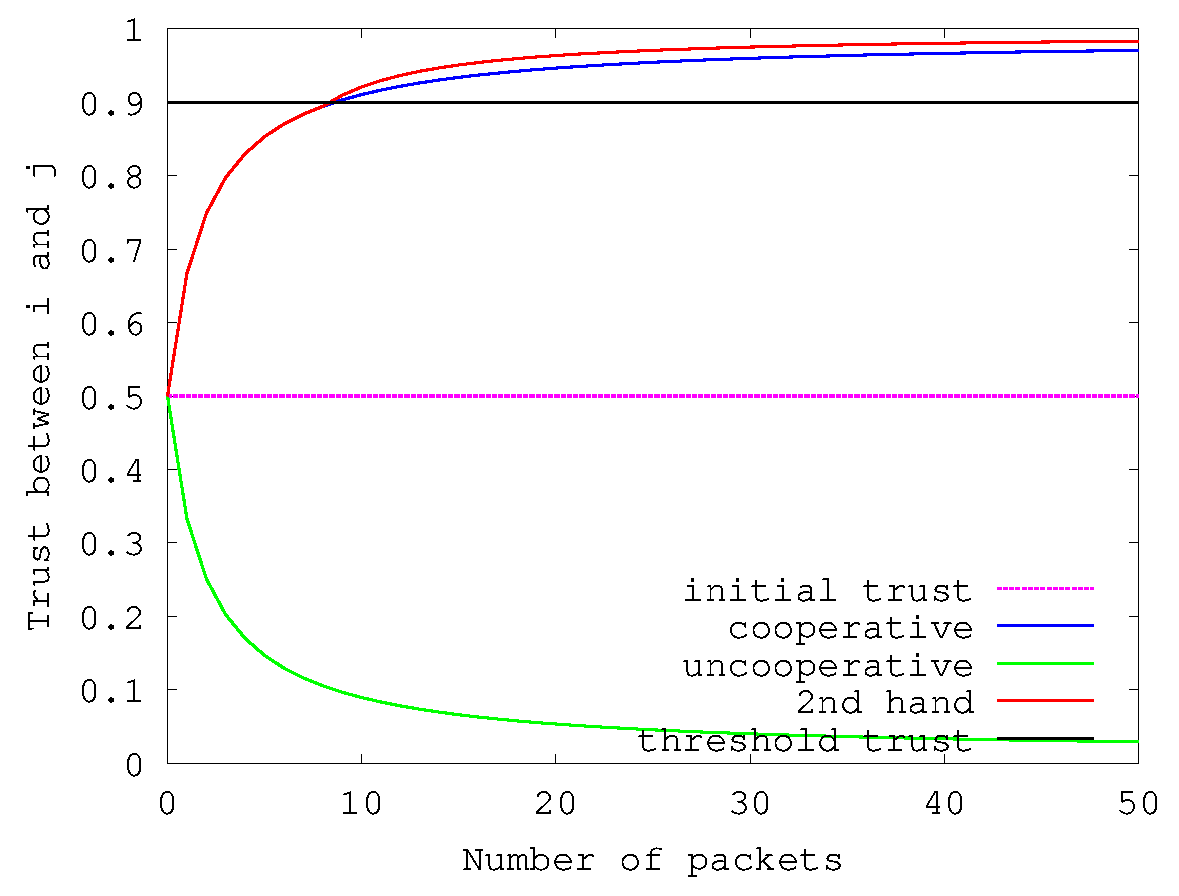
\includegraphics[width=.9\linewidth]{./resources/reputation-paper.eps}
  \caption{Co\"operatieve en niet-co\"operatieve knopen}
  \label{fig:reputation-paper}
\end{subfigure}
\begin{subfigure}{.49\textwidth}
  \centering
  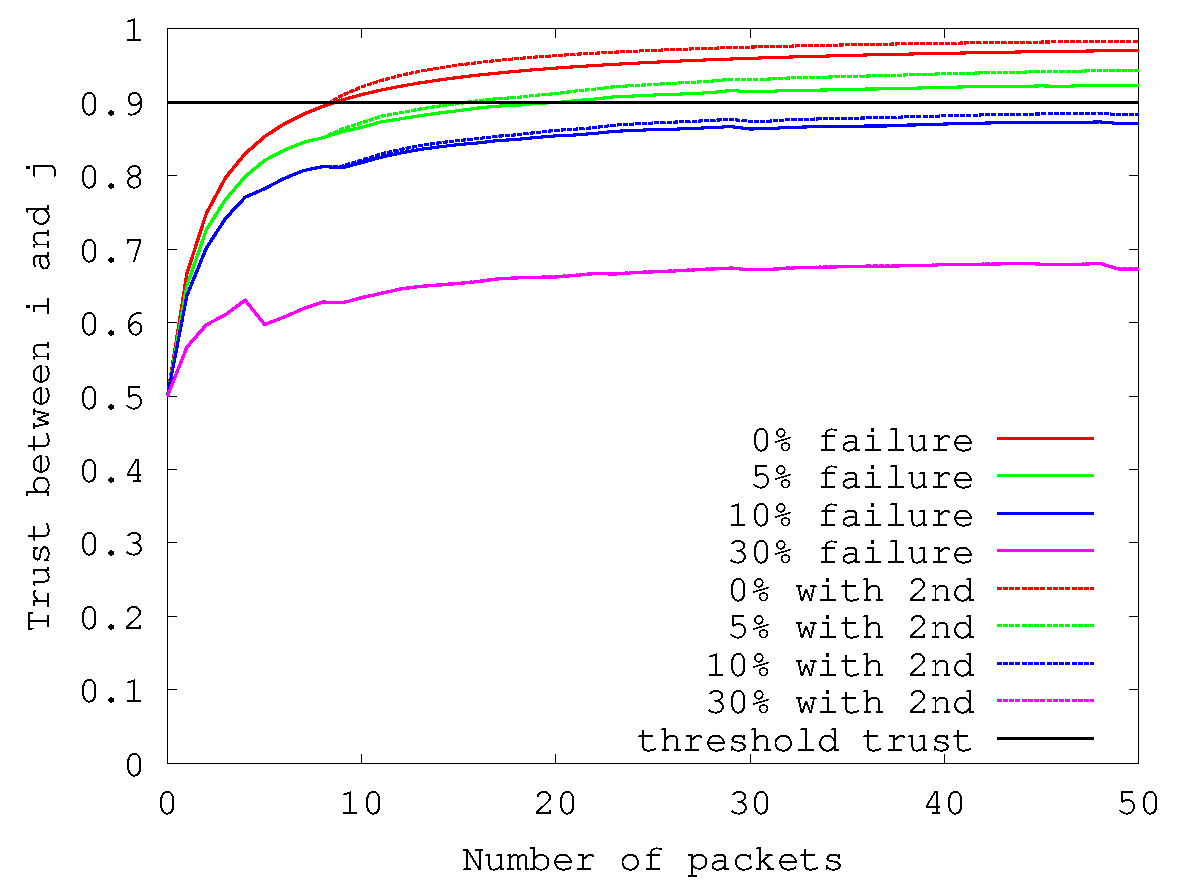
\includegraphics[width=.9\linewidth]{./resources/reputation-with-failure.eps}
  \caption{Falende knopen (100 simulaties)}
  \label{fig:reputation-with-failure}
\end{subfigure}
\caption{Impact van falende knopen op evolutie van vertrouwen.}
\label{fig:reputation-paper-with-failure}
\end{figure}

Deze eigenschap kan echter misbruikt worden zoals aangetoond wordt in figuur
\ref{fig:reputation-with-failure}. Stel dat een knoop $j$ te kampen heeft met
falende hardware, waardoor 5\% van zijn transmissies verloren gaan en daarom
ook niet opgemerkt kunnen worden door andere knopen.

We merken op dat deze knoop, zelfs met 5\% niet-co\"operatieve observaties, na
een twintigtal observaties toch boven de drempelwaarde uitkomt en door de
beschouwende knoop aanvaard wordt als betrouwbaar.

Vanuit een operationeel standpunt gezien is dit in eerste instantie een
positief effect. Indien een node \emph{slechts} 5\% faalt zal deze toch als
co\"operatief beschouwd worden en de goede werking van het netwerk niet
fundamenteel in het gedrang brengen - vanuit een inbraakdetectie oogpunt gezien.

Maar stel dat deze 5\% niet-co\"operatieve acties geen falen zijn en dat de
doorgestuurde boodschappen niet verloren gaan, maar met opzet lichtjes
gewijzigd worden. 5\% kan een significante vertekening van metingen van een
netwerk betekenen en zo de werking van het hele netwerk ondermijnen.

\TODO example of well-crafted malicious behavior

\TODO

\cite{krontiris2009cooperative,castelluccia2009difficulty,krauss2007detecting,seshadri2008sake,maerien2012famos,aschenbruck2012security,afzal2012difisec,yue2012novel,kuang2010snds,blilat2012wireless,ramesh2012wireless,valero2012di,perrig2004security,zhang2000intrusion,djenouri2005survey,yu2008framework,rassam2011novel,da2005decentralized,kachirski2003effective,li2008group,mishra2004intrusion,krontiris2008lidea,ioannis2007towards,soliman2012comparative,wang2011integrated,zhijie2012intrusion}

%%!TEX root=masterproef.tex
\chapter{Besluit}
\label{besluit}

\chapterprecishere{
At least for the people who send me mail about a new language that they're
designing, the general advice is: do it to learn about how to write a compiler.
Don't have any expectations that anyone will use it, unless you hook up with
some sort of organization in a position to push it hard. It's a lottery, and
some can buy a lot of the tickets. There are plenty of beautiful languages
(more beautiful than C) that didn't catch on. But someone does win the lottery,
and doing a language at least teaches you something.
\par\raggedleft--- \textup{Dennis Ritchie (1941-2011)},\\
Creator of the C programming language and of UNIX}

% De masterproeftekst wordt afgesloten met een hoofdstuk waarin alle
% besluiten nog eens samengevat worden. Dit is ook de plaats voor suggesties
% naar het verder gebruik van de resultaten, zowel industri\"ele toepassingen
% als verder onderzoek.

\TODO

\section{Sterke punten}
\label{section:strenghts}

\TODO

\section{Zwakke kanten}
\label{section:weaknesses}

\TODO

\section{Opportuniteiten}
\label{section:opportunities}

\TODO

\section{Bedreigingen}
\label{section:threaths}

\TODO

\section{De slotsom}
\label{section:bottom-line}

\TODO

\begin{figure}[ht]
  \centering
  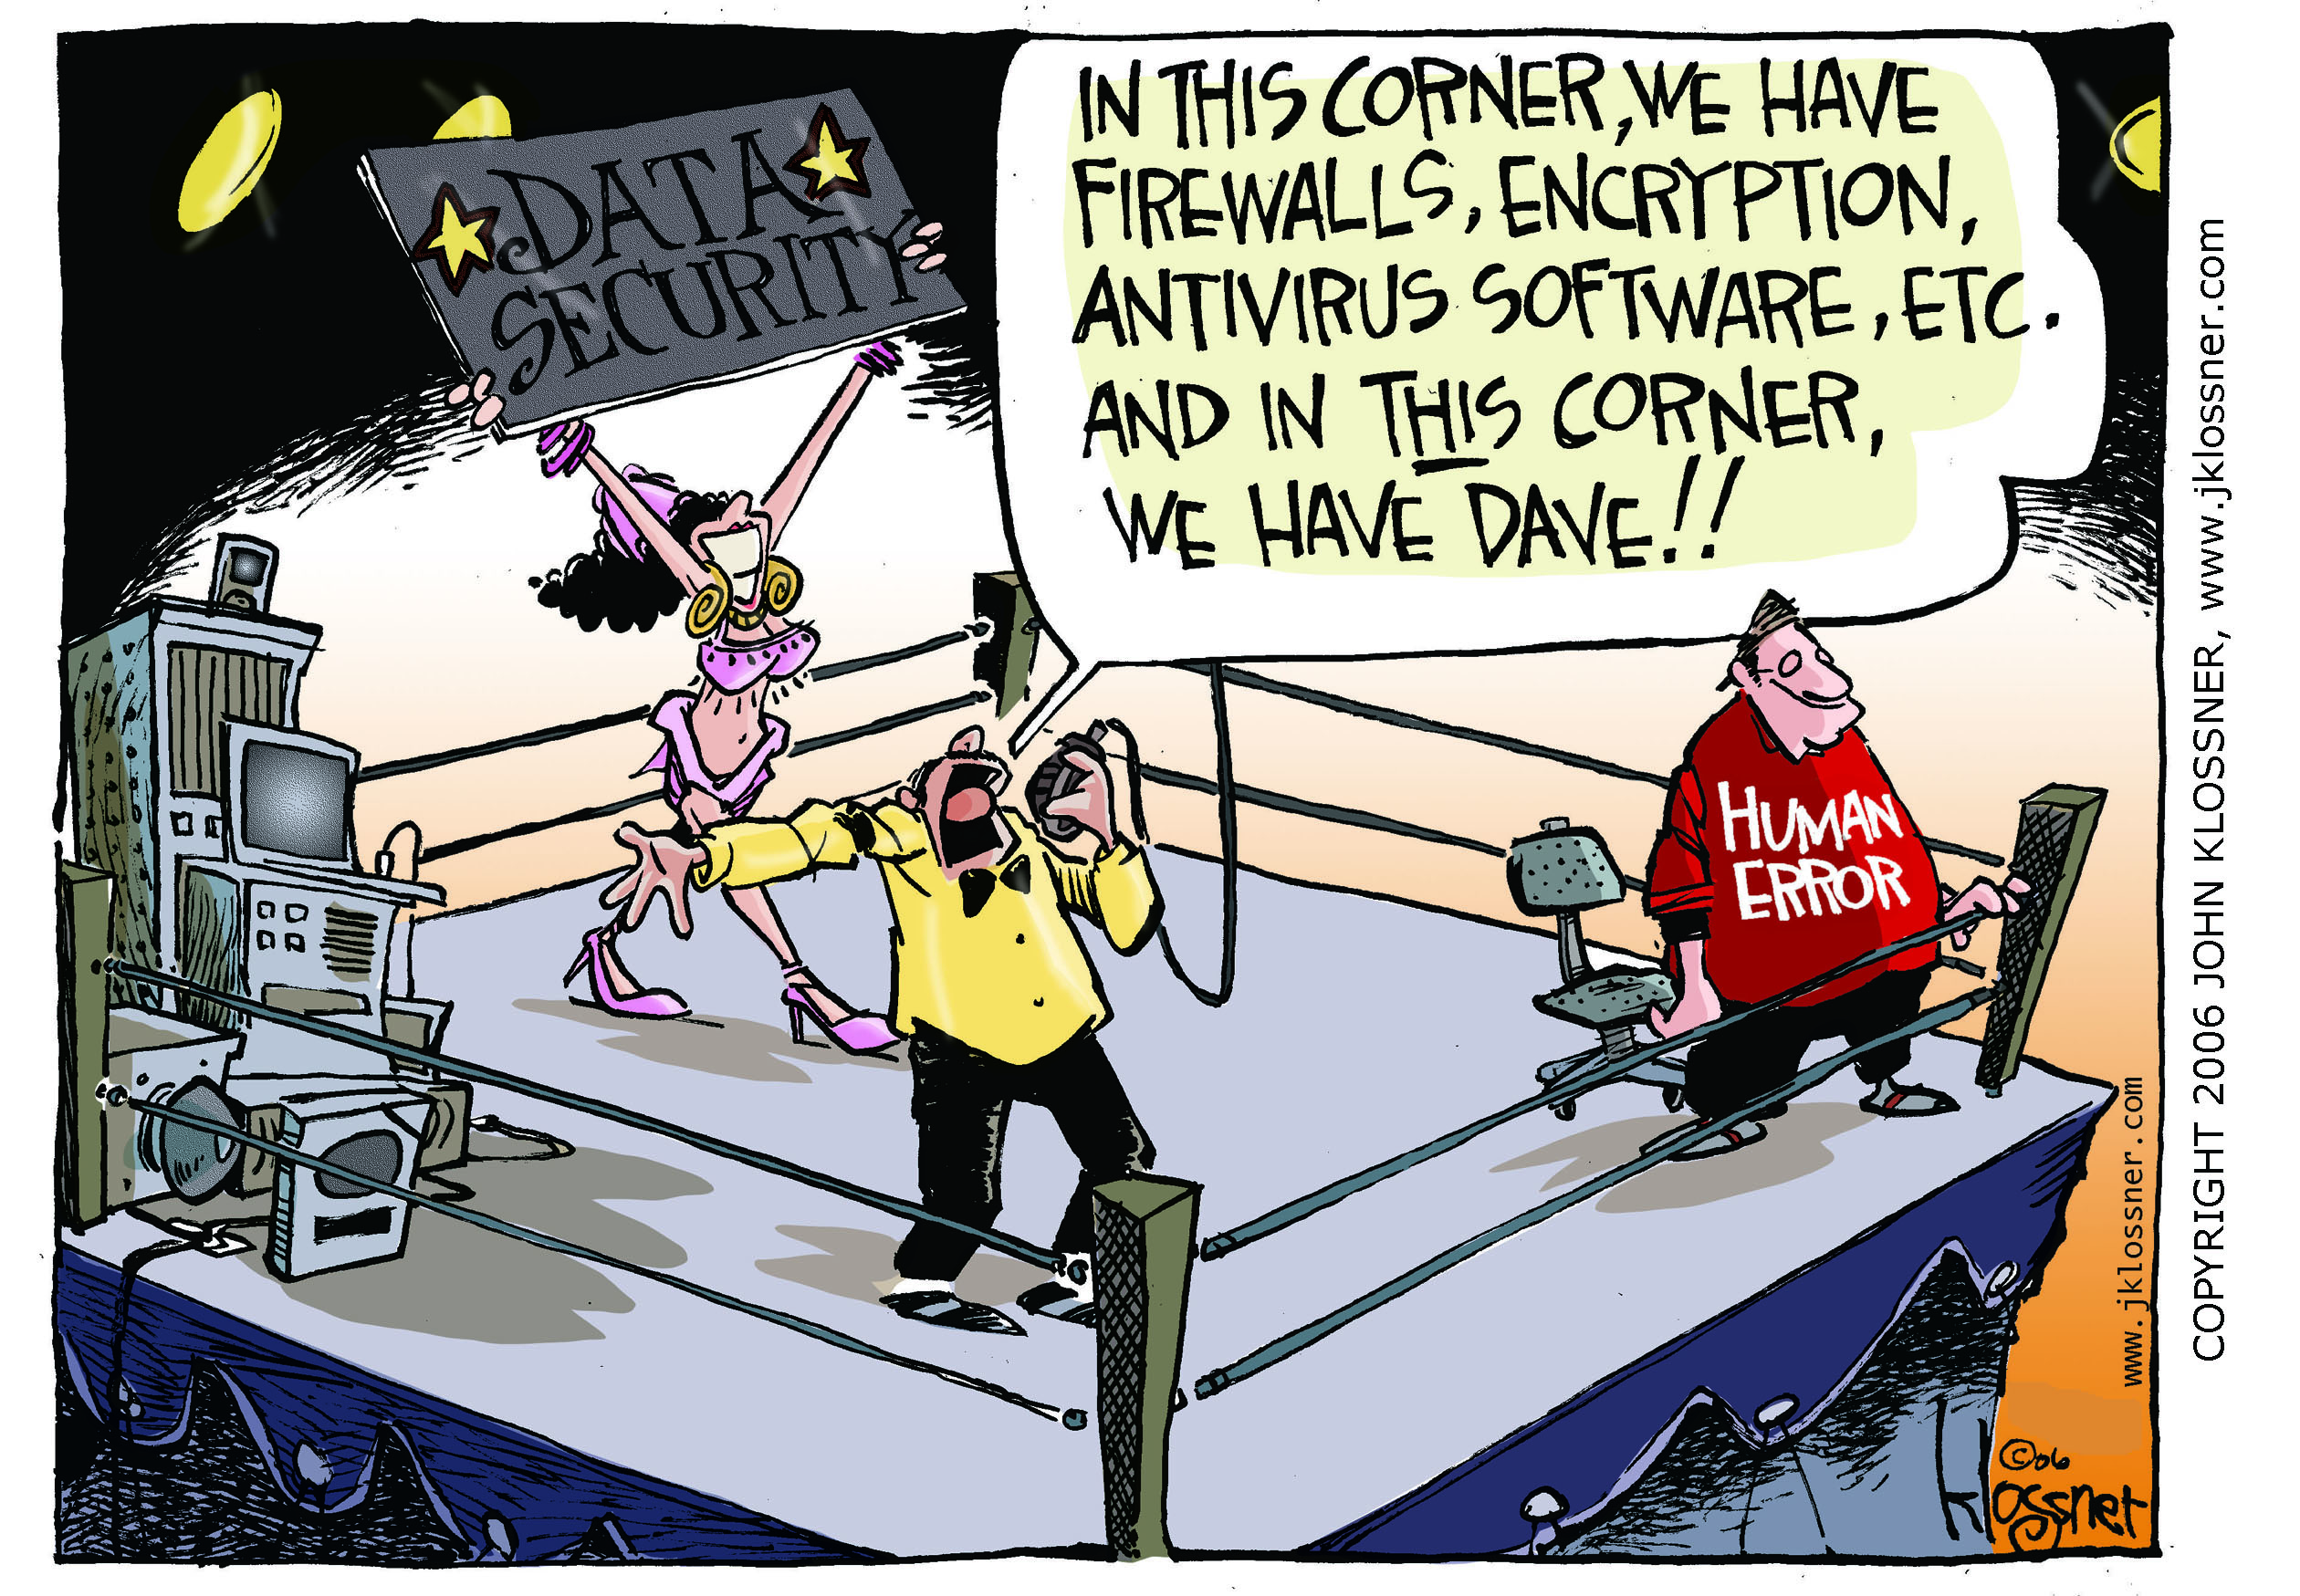
\includegraphics[width=\linewidth]{resources/cartoon_human_error.jpg}
  \caption[``Human Error'']{``Human Error'' - courtesy of John Klossner}
\end{figure}


% TODO:

% Het feit dat in essentie een nieuwe taal was, bracht ook een bijkomende
% leercurve met zich mee. Ook zorgde voortschrijdend inzicht voor stapsgewijze
% verbeteringen aan bepaalde constructies, die echter soms door tijdbeperkingen
% niet voor alle overige code konden bijgewerkt worden.



%\appendixpage*
%\appendix
%\chapter{De eerste bijlage}
\label{app:A}
In de bijlagen vindt men de data terug die nuttig kunnen zijn voor de
lezer, maar die niet essentieel zijn om het betoog in de normale tekst te
kunnen volgen. Voorbeelden hiervan zijn bronbestanden,
configuratie-informatie, langdradige wiskundige afleidingen, enz.

In een bijlage kunnen natuurlijk ook verdere onderverdelingen voorkomen,
evenals figuren en referenties\cite{h2g2}.

\section{Meer lorem}
\lipsum[50]

\subsection{Lorem 15--17}
\lipsum[15-17]

\subsection{Lorem 18--19}
\lipsum[18-19]

\section{Lorem 51}
\lipsum[51]

%%% Local Variables: 
%%% mode: latex
%%% TeX-master: "masterproef"
%%% End: 


%\backmatter

\bibliographystyle{abbrv}
\bibliography{referenties}

\end{document}
